% -----------------------------------------------
% Template for ISMIR Papers
% 2017 version, based on previous ISMIR templates
% Requirements :
% * 6+n page length maximum
% * 4MB maximum file size
% * Copyright note must appear in the bottom left corner of first page
% * Clearer statement about citing own work in anonymized submission
% (see conference website for additional details)
% -----------------------------------------------

\documentclass{article}
\usepackage{ismir,amsmath,cite,url}
\usepackage{graphicx}
\usepackage{color}

% Title.z
\title{Modeling The Complexity of Music Metadata in Semantic Graphs for Exploration and Recommendation}

% Note: Please do NOT use \thanks or a \footnote in any of the author markup

% Single address
% To use with only one author or several with the same address
% ---------------
%\oneauthor
% {Names should be omitted for double-blind reviewing}
% {Affiliations should be omitted for double-blind reviewing}

% Two addresses
% --------------
%\twoauthors
%  {First author} {School \\ Department}
%  {Second author} {Company \\ Address}

%% To make customize author list in Creative Common license, uncomment and customize the next line
%  \def\authorname{First Author, Second Author}


% Three addresses
% --------------
% \threeauthors
%   {Pasquale Lisena} {EURECOM, France \\ {\tt pasquale.lisena@eurecom.fr}}
%   {Rapha\"el Troncy} {EURECOM, France \\ {\tt raphael.troncy@eurecom.fr}}
%   {Konstantin Todorov} {LIRMM, University of Montpellier, France \\ {\tt konstantin.todorov@lirmm.fr}}

\threeauthors
  {First Author} {Affiliation1 \\ {\tt author1@ismir.edu}}
  {Second Author} {\bf Retain these fake authors in\\\bf submission to preserve the formatting}
  {Third Author} {Affiliation3 \\ {\tt author3@ismir.edu}}

%% To make customize author list in Creative Common license, uncomment and customize the next line
%  \def\authorname{First Author, Second Author, Third Author}

% Four or more addresses
% OR alternative format for large number of co-authors
% ------------
%\multauthor
%{First author$^1$ \hspace{1cm} Second author$^1$ \hspace{1cm} Third author$^2$} { \bfseries{Fourth author$^3$ \hspace{1cm} Fifth author$^2$ \hspace{1cm} Sixth author$^1$}\\
%  $^1$ Department of Computer Science, University , Country\\
%$^2$ International Laboratories, City, Country\\
%$^3$  Company, Address\\
%{\tt\small CorrespondenceAuthor@ismir.edu, PossibleOtherAuthor@ismir.edu}
%}
%\def\authorname{First author, Second author, Third author, Fourth author, Fifth author, Sixth author}

\sloppy % please retain sloppy command for improved formatting

%%%%%%%%%%%%%%%%%%%%%%%%%%%%%%%
%%%  Beginning of document  %%%
%%%%%%%%%%%%%%%%%%%%%%%%%%%%%%%

\begin{document}

\maketitle

%%%%%%%%%%%%%%%%%%
%%%  Abstract  %%%
%%%%%%%%%%%%%%%%%%

\begin{abstract}
% The abstract should be placed at the top left column and should contain about 150-200 words.
Representing and retrieving fine-grained information related to something as complex as music composition, recording and performance is a challenging activity. This complexity requires that the data model enables to describe different outcomes of the creative process, from the writing of the score, to its performance and publishing. In this paper, we show how we design the DOREMUS ontology as an extension of the FRBR model in order to represent music metadata coming from different libraries and cultural institutions and how we publish this data as RDF graphs. Controlled vocabularies provide common thesauri that overcome the differences in language and alternative forms. These graphs are interlinked to each other and to external resources on the Web of Data. We show how these graphs can be walked through for designing a web-based application providing an exploratory search engine for presenting complex music metadata to the end-user. Finally, we demonstrate how this model and this exploratory application is suitable for answering non-trivial questions collected from experts and is a first step towards a fully fledged recommendation engine.
\end{abstract}

%%%%%%%%%%%%%%%%%%%%%%%%%
%%%  1. Introduction  %%%
%%%%%%%%%%%%%%%%%%%%%%%%%

\section{Introduction}\label{sec:introduction}
Music metadata can be very complex. Metadata about a well-known masterpiece such as the \textit{Moonlight Sonata} can include a description of its composition by Beethoven, its scores in the handmade or printed version, some interpretations by pianists, the orchestrations and arrangements. Performances, recordings, music albums can also be described and attached to this work. Numerous actors are involved in this media production chain: composers, performers with their own different roles, conductors, {\it etc.}

An even more challenging tasks consist in describing jazz and ethnic music for which the performance plays a central role. In jazz, each improvisation can be considered as a creation event of a new expression, of which the performer is the author. In ethnic music, the absence of a score and a composer as in classical western music implies the need for a different way of describing it.

Libraries have plenty of structured information that is currently encoded in different formats such as relational tables, XML, CSV and very specialized ones like MARC\footnote{\url{https://www.loc.gov/marc/}} and its variants. This heterogeneity is not satisfactory for different reasons. Often, the structure of the data is guided by a set of arbitrary rules, which are internal to each institution and can have non-explicit semantics, making hard the understanding of the model. Furthermore, some popular musical works are described by different catalogs with complementary and overlapping metadata. Discovering duplicates and performing a reconciliation and interconnection of the data will produce enriched information that will combine the knowledge coming from different data sources. In its current state, music metadata has little chances of effortless and automatic reconciliation and linking. Finally, these formats are not ready to be directly consumed by applications for visualization, exploration and recommendation. They require significant parsing efforts and semantic interpretation which deter their full potential usage. We observe that musical institutions are constantly more interested in automatic support for the editorial work of making the programme for a concert or a musical playlist for a radio. This help can come from a recommendation system that shall reveal otherwise unknown works from the huge amount of data available.

In this paper, we give an overview of our efforts and current results in harmonizing the musical data coming from three leading cultural institutions in France --- the BnF (Biblioth\`eque Nationale de France), the Philharmonie de Paris (PP) and Radio France (RF). Our research contributions include: a new powerful model based on FRBR for describing music metadata in its complexity (Section~\ref{sec:model}); tools for converting legacy metadata in semantic graphs and a novel algorithm enabling to deduplicate music entities (Section~\ref{sec:conversion-linking}); a web-based exploratory search engine that validates the model in demonstrating how complex user needs can be answered for the first time (Section~\ref{sec:exploration}).

%%%%%%%%%%%%%%%%%%%%%%%%%
%%%  2. Related Work  %%%
%%%%%%%%%%%%%%%%%%%%%%%%%

\section{Related Work}\label{sec:related-work}
Semantic Web technologies emerged in the field of data management with the ambitious promise to realise the \textit{Web of Data}. The latter can be seen as a set of interconnected datasets in the form of graphs, in which the information is represented through triples of the form ``subject-predicate-object'', following the Resource Description Framework (RDF) data model. Each resource is identified by a URI (Unique Resource Identifier) that can be accessed for obtaining information about the resource itself. Properties are also identified by URIs, making it possible to attach to each of them labels and descriptions, for making the understanding and the adoption of a particular ontology easier.

The management of music-related information through the Semantic Web has lead to the creation of the Music Ontology~\cite{raimond2007music}, that provides a set of music-specific classes and properties for describing musical works, performances and tracks, together with fragments of them. The authors foresee the use of taxonomies and vocabularies for populating the values of certain properties, like keys, instruments and genres. Several examples of interconnecting Music Ontology to other datasets, whether they describe music or other kind of data, like DBpedia, are shown in~\cite{raimond2008webmusic}.

The role of a taxonomy of musical instruments in complex query answering is investigated in \cite{kolozali2011knowledge}, demonstrating that the RDF structure helps reasoning engines to discover links between different levels in the hierarchy of instruments. The need for harmonization of musical metadata coming from different sources with different formats led to different technical solutions, often making use of Semantic Web technologies. One of them could be a service that stands between the data and the consumers and that performs real-time conversion of each query to source-specific queries, the consequent conversion of each result in a common format and their combination, without needs for pre-processing~\cite{lai2007metadata}. In some cases, this approach can be impossible to realise because the structure of certain documents is not suitable for all kinds of queries. Another strategy relies on converter tools based on static mapping. This strategy often foreseen an alignment to be performed after the conversion, for discovering co-references between sources, like in \cite{bretherton2009integrating}, when a faceted search interface for accessing the data is also described. 

Semantic Web technologies allows also to perform recommendation using the graph structure. Among existing approaches,~\cite{braunhofer2013location} proposes to compute the shortest walk in the graph~\cite{braunhofer2013location} while~\cite{rosati2016rdf} builds embedding of entities for computing their similarity.

%%%%%%%%%%%%%%%%%%%%%%%%%%%
%%%  3. Modeling Music  %%%
%%%%%%%%%%%%%%%%%%%%%%%%%%%

\section{Modeling Music}\label{sec:model}
In this section, we describe a data model for music metadata: the DOREMUS ontology and a set of controlled vocabularies that we selected, formalized and finally interlinked.

\subsection{Ontology}\label{subsec:onto}
The Semantic Web is often making use of ontologies for making explicit the semantics of the data. The description of music is historically connected to catalog information models, among which FRBR is one of the most popular. FRBR and CIDOC-CRM, an ontology for describing museum information, have been harmonized in the FRBRoo model for describing arts~\cite{doerr2008frbroo}. This is a dynamic model, in which the abstract intention of the Work exists only through its Creation Event that realises it in a distinct series of choices called Expression. This Work-Expression-Event triplet can describe also different parts of the life of a work, like the Performance, the Publication or a derivative Work, each one incorporating the expression from which it comes from.

The DOREMUS model\footnote{\url{http://data.doremus.org/ontology/}}, with its default prefix \texttt{mus}, is an extension of FRBRoo for the music domain. On top of its original classes and properties, specific ones have been added in order to describe aspects of a work that are specifically related to music, such as the musical key, the genre, the tempo, the medium of performance, {\it etc.}~\cite{choffe2016doremus}. The triplet pattern of FRBRoo ensures that each step of the life of a musical work can be modelled separately. For this reason, the composition and the performance, the score and the recording have in DOREMUS the same importance and each contain an information that in the same time can live autonomously and be linked to the other entities.

\subsection{Controlled vocabularies}
A large number of properties that are involved in the music description are supposed to contain values that are shared among different entities: different composition can have as genre ``sonata'', different performer can play a ``bassoon'', different authors can have as function ``composer'' or ``lyricist''. These labels can be expressed in multiple languages or in alternative forms (i.e. ``sax'' and ``saxophone''), making reconciliation hard. Our choice is to use controlled vocabularies for each category of concepts. A controlled vocabulary is a thematic thesaurus of entities, each one being again identified with a URI. We are using SKOS, that allows to specify for each Concept the preferred and the alternative labels in each language, to define a hierarchy between them (so that the ``violin'' is a narrower concept with respect to ``string''), and to add comments and notes for describing the entity and help the annotation activity. Each concept becomes a common node in the musical graph that can related two musical works, two authors or performers.

Different kinds of vocabularies are needed for describing music: some are already available on the web (such as medium of performance\footnote{\url{http://iflastandards.info/ns/unimarc/terms/mop/}} or musical genres\footnote{\url{http://iflastandards.info/ns/unimarc/terms/fom/}}, while others do not exist (like the types of derivation). Not all of them are published in a suitable format for the Web of Data, and there is often little correspondences between vocabularies. We published until now 15 controlled vocabulary belonging to 7 different categories, while others are going to be realised. %The definition of appropriate relationships and mappings between the different sources is being realised (TODO write the status of vocabulary interconnection).

\subsection{Vocabulary Alignment}
In each category of vocabularies (e.g., medium of performance (MoP), genres), we have identified and skosified a set of vocabularies that are originally used by our three partner institutions. In order to ensure data interoperability, these vocabularies need to be aligned, by establishing the equivalence relations between their corresponding classes (e.g., knowing that ``cha cha cha'' from a genre vocabulary corresponds to ``cha-cha-cha`'' used by the French BnF library). Given the sizes of these thesauri, sometimes reaching several thousands of terms, this process needs to be assisted by an automatic matching tool. We have relied on the YAM++ system\footnote{\url{http://yamplusplus.lirmm.fr/index}}, that has shown to perform well on generic ontology matching tasks in past years OAEI evaluations. Its particularity is that it goes beyond string matching, by exploring the structure and the semantic context of the two input vocabularies. We have developed a web platform that allows the librarian experts to visualize and manually validate and enrich the automatically produced vocabulary alignments\footnote{\url{http://yamplusplus.lirmm.fr/validator}}. In this way, a (hopefully) large pool of matching vocabulary terms is produced automatically, but the domain experts have the final say. Currently, five genre-related vocabularies six MoP-vocabularies have been automatically aligned and validated by domain-experts.

%%%%%%%%%%%%%%%%%%%%%%%%%%%%%%%%%%%%%%%%
%%%  4. Data Conversion and Linking  %%%
%%%%%%%%%%%%%%%%%%%%%%%%%%%%%%%%%%%%%%%%

\section{Data Conversion and Linking}
\label{sec:conversion-linking}
The benefits of moving from MARC to an RDF-based solution consist in the interoperability and the integration among libraries and with third part actors, with the possibility of realizing smart federated search~\cite{byrne2010strongest}. The realisation of these goals pass by two main tasks: data conversion and data linking.

\subsection{From MARC to RDF}
The archives of librarian institution like BnF and the Philharmonie de Paris (PP) are used to describe music in the MARC format, that consists in a succession of fields and subfields, identified by their own code, as shown in \figref{fig:unimarc}. The semantics of these fields and subfields is not trivial: a subfield can change its meaning depending on the field, under which it is found, and on the particular variant of MARC (UNIMARC and INTERMARC). A field or subfield can contain information about different entities, like the first performance and the first publication mixed up in the same field of the notes. Often, the information is represented in the form of a human-readable string, so that Natural Language Proceessing (NLP) techniques are needed for extracting it.

We rely on {\smallsc marc2rdf}\footnote{\url{https://github.com/DOREMUS-ANR/marc2rdf}}, an open source prototype for the automatic conversion of MARC bibliographic records to RDF, implementing the DOREMUS model~\cite{lisena2016exploring}. The conversion process relies on explicit expert-defined transfer rules (or mappings) that indicate where in the MARC file to look for what kind of information, providing the corresponding property path in the model as well as useful examples that illustrate each transfer rule, as shown in \figref{fig:mappings}. Moreover, a knowledge-aware parsing on the text notes is performed in order to further extract information from strings (i.e. extracting the medium of performance from the casting notes, or the date from the first publication note). Resources are identified by URIs that use the corresponding DOREMUS class labels in their names (as for example \url{http://data.doremus.org/expression/UUID} identifying an instance of the FRBRoo class \texttt{Expression}). The software contains also a \smallsc{string2uri} component, inspired by the Datalift platform~\cite{scharffe2012enabling}, that performs an automatic mapping of string literals to URIs coming from controlled vocabularies.

\begin{figure}
 \centerline{\framebox{
  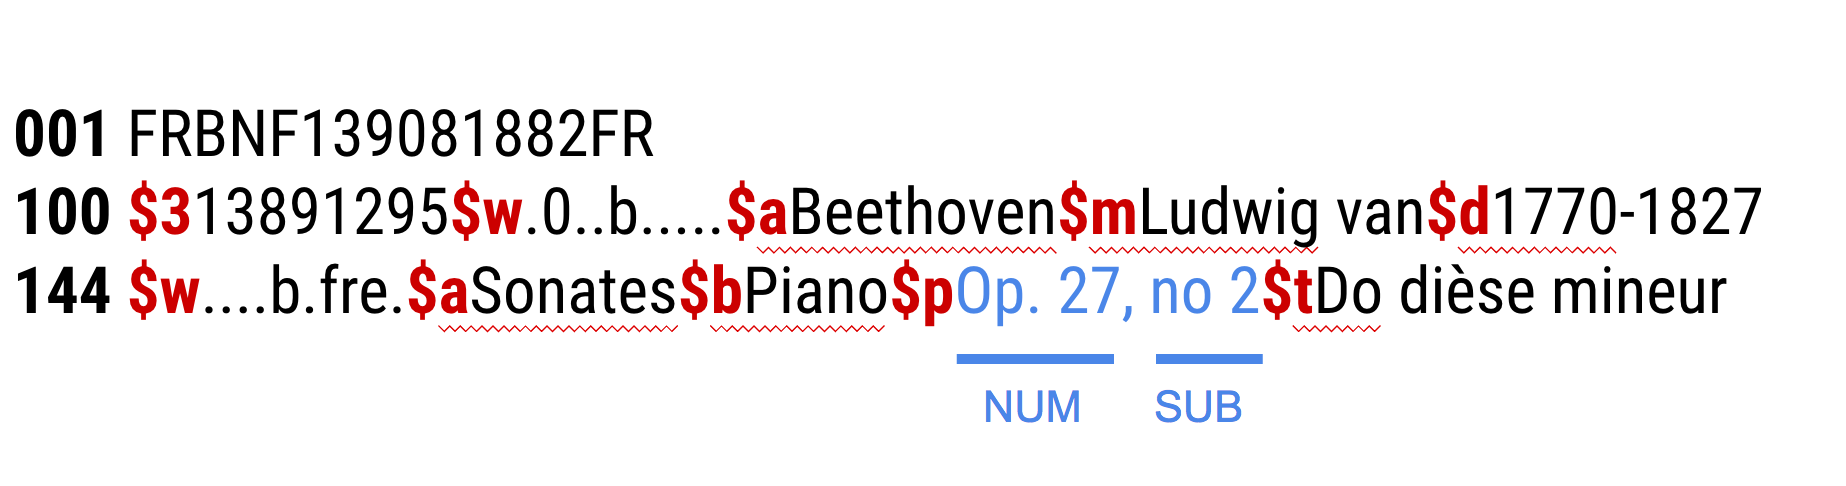
\includegraphics[width=6cm]{figs/MARC_example.png}}}
  \caption{An excerpt of a UNIMARC record.}
 \label{fig:unimarc}
 \smallskip
 \centerline{\framebox{
  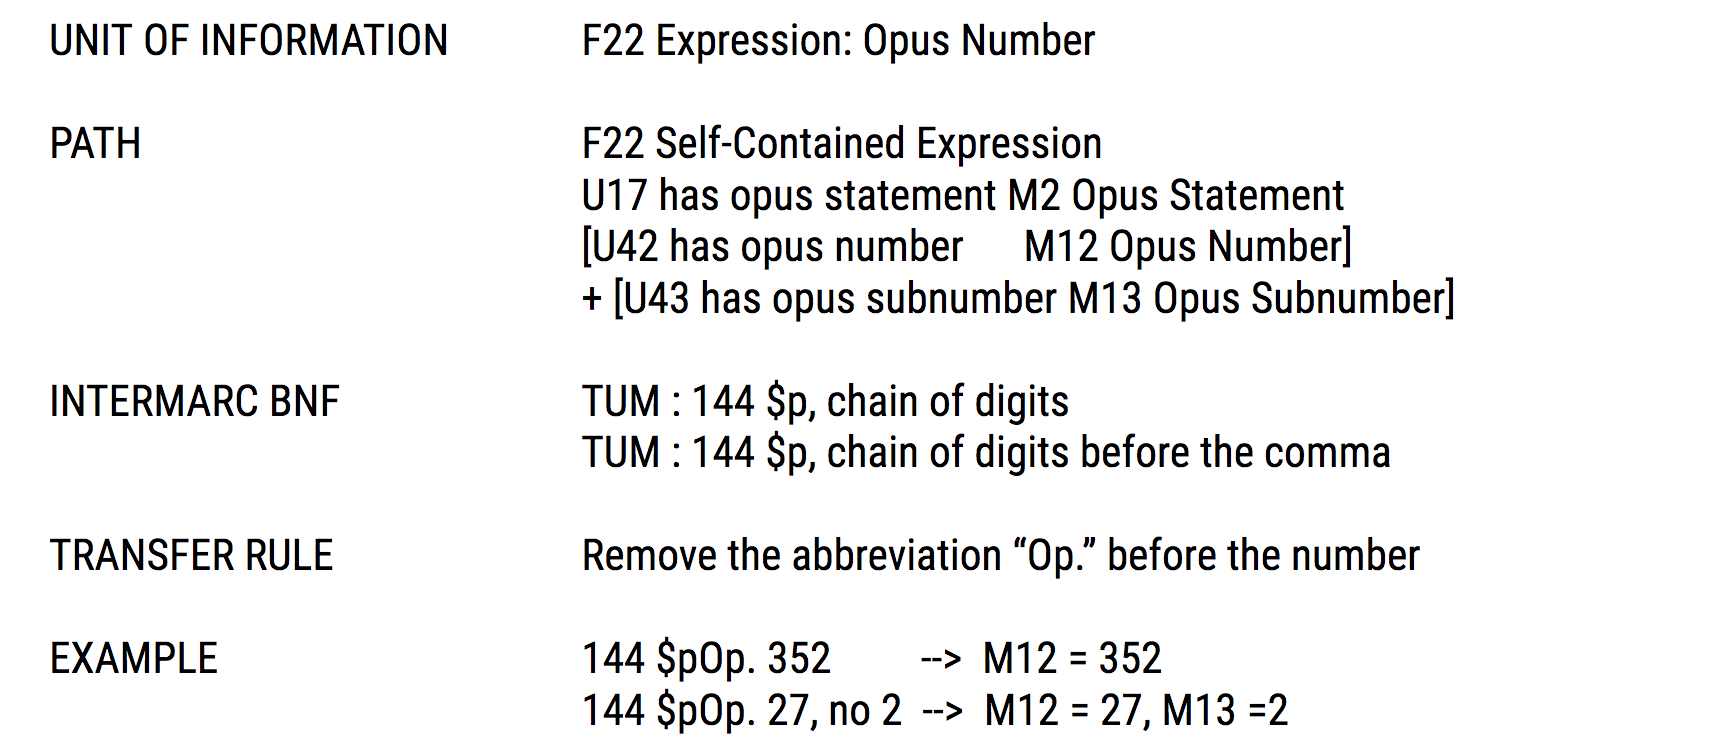
\includegraphics[width=\columnwidth]{figs/mapping_rule.png}}}
  \caption{Example of mapping rules describing the opus number and sub-number of a work}
 \label{fig:mappings}
\end{figure}

\begin{figure}
 \centerline{
 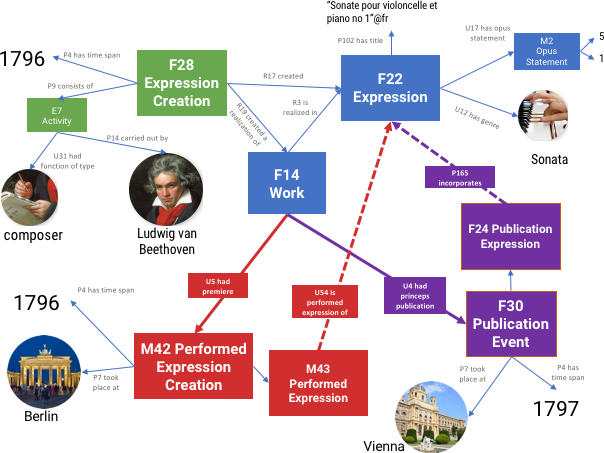
\includegraphics[width=\columnwidth]{figs/schema.png}}
 \caption{Beethoven's \textit{Sonata for piano and cello n.1} represented as a graph}
 \label{fig:schema}
\end{figure}

\subsection{Example as a graph}
The graph depicted in \figref{fig:schema} shows an example taken from the converted data: Beethoven's \textit{Sonata for piano and cello n.1}\footnote{\url{http://data.doremus.org/expression/614925f2-1da7-39c1-8fb7-4866b1d39fc7}}. The FRBRoo triplet contains all the information about the work and its composition by Beethoven. Then, the information about the performance and publication are linked to the triplet through specific properties. The nodes represented as circles consist normally in URIs taken from controlled vocabularies (the function ``composer'' or the genre ``sonata'') or are entities that are matched to external datasets (the person of Beethoven or the places Berlin and Vienna). Each one of these nodes can represent a link between different works, performances, etc., making everything connected in a large graph.  

\subsection{Data Linking} \label{subsec:datalinking}
The {\smallsc marc2rdf} prototype allows to transform a MARC dataset to RDF using the DOREMUS model. If we take again the example of the BnF and the Philharmonie institutions, we end up with two RDF graphs sharing a large number of entities, such as music works or creation events. Therefore, a crucial task in order to enable the interoperability between these datasets and allow to navigate through them and explore them, is the task of data linking (or link discovery), defined as establishing identity relations between the elements of these graphs in a (mostly) automated manner. Firstly, we focus on matching music works across datasets. However, due to the high data heterogeneity in the musical field, link discovery becomes a challenging task. These heterogeneities include important structural, syntactic and lexical differences in descriptions of musical works, use of different languages or titles, to name a few. To train and test data linking tools, we have collected benchmark data from those institutions as part of the 2016 OAEI instance matching evaluation campaign\footnote{\url{http://islab.di.unimi.it/content/im_oaei/2016/#doremus}}.

Our initial tests with off-the-shelf linking tools, such as SILK\footnote{\url{http://silkframework.org}} did not show satisfactory results. We have, therefore, developed a novel linking system, named LEGATO, designed to handle the richness and diversity of music data. On the one hand, LEGATO puts a special emphasis on the pre-processing phase which allows to filter out problematic properties containing long human readable strings in the form of comments. On the other hand, the tool allows to repair erroneous mappings before producing the final linkset, by using clustering and key-discovery techniques. In addition, LEGATO is well-suited to users with little or no technical knowledge of the linking process, since it requires very little configuration, in contrast to most state-of-the-art tools \cite{nentwig2015survey}. In Section~\ref{sec:eval-link}, we show results of evaluating LEGATO against the popular link discovery tool SILK.

%%%%%%%%%%%%%%%%%%%%%%%%%%%%%%%%%%%%%%%%%%
%%%  5. Music Discovery with Overture  %%%
%%%%%%%%%%%%%%%%%%%%%%%%%%%%%%%%%%%%%%%%%%

\section{Music Discovery with Overture}
\label{sec:exploration}
We developed the first version of \textsc{Overture} (Ontology-driVen Exploration and Recommendation of mUsical REcords), a prototype of an exploratory search engine for DOREMUS data. \textsc{Overture} is developed as a modern web app, implemented with Node.JS and Angular and available at \url{http://overture.doremus.org}. The application make requests directly to our SPARQL endpoint\footnote{\url{http://data.doremus.org/sparql}} and provide the information to the end-user with a nice interface. %So far, only the part of expression is fully complete, while the other section are under development.

\subsection{Visualizing the complexity}
On the top of the user interface, the navigation bar allows the user to navigate between the main concepts of the DOREMUS model: expression, performance, score, recording, artist. The challenge is in giving to the final user a complete vision on the data of each class and letting him/her to understand how they are connected to each other. \figref{fig:overture-detail} represents Beethoven's \textit{Sonata for piano and cello n.1}. Aside from the different versions of the title, the composer and a textual description, the page provides details on the information we have about the work, like the musical key, the genres, the intended medium of performance, the opus number. When these values come from a controlled vocabulary, a link is present in order to search for the expression that share the same value, for example, the same genre or the same musical key. A timeline shows the most important events in the story of the work (the composition, the premiere, the first publication). Other performances and publications can be represented below.

\begin{figure}
 \centerline{
 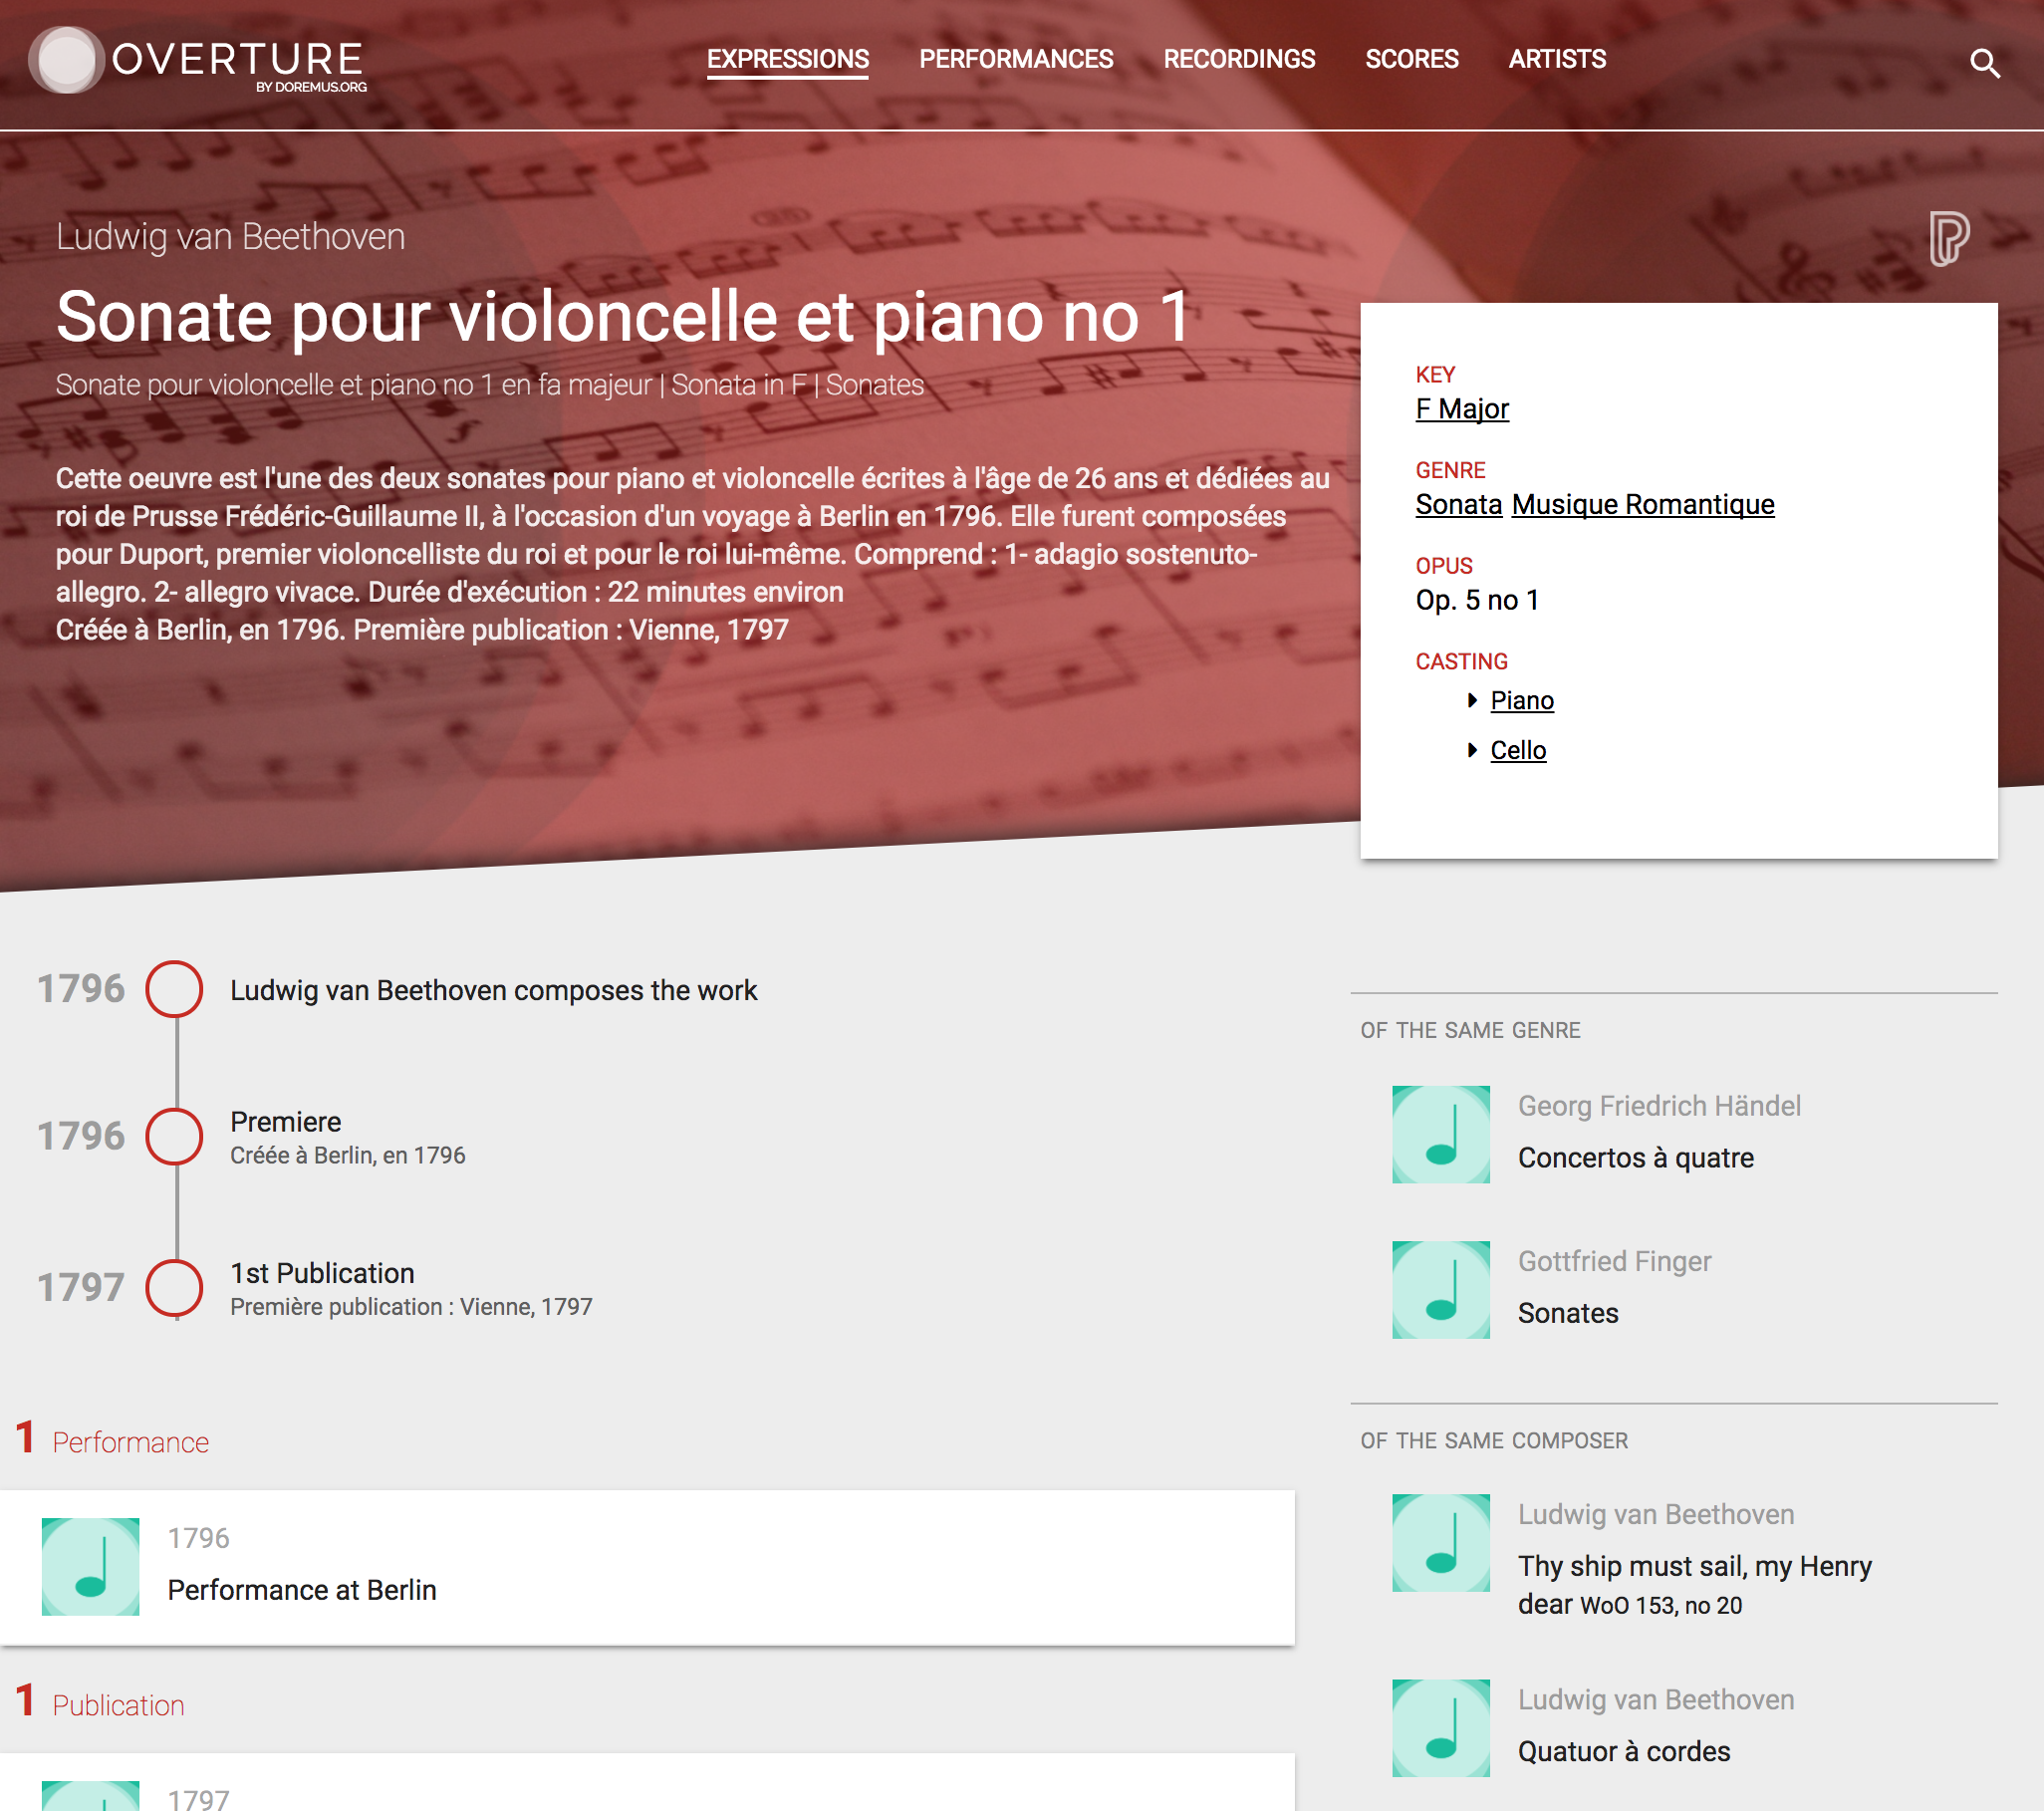
\includegraphics[width=\columnwidth]{figs/overture-sonate-cello.png}}
 \caption{The detail of an expression in \textsc{Overture}}
 \label{fig:overture-detail}
\end{figure}

\subsection{Explore and recommend}
% \begin{figure}
%  \centerline{\framebox{
%  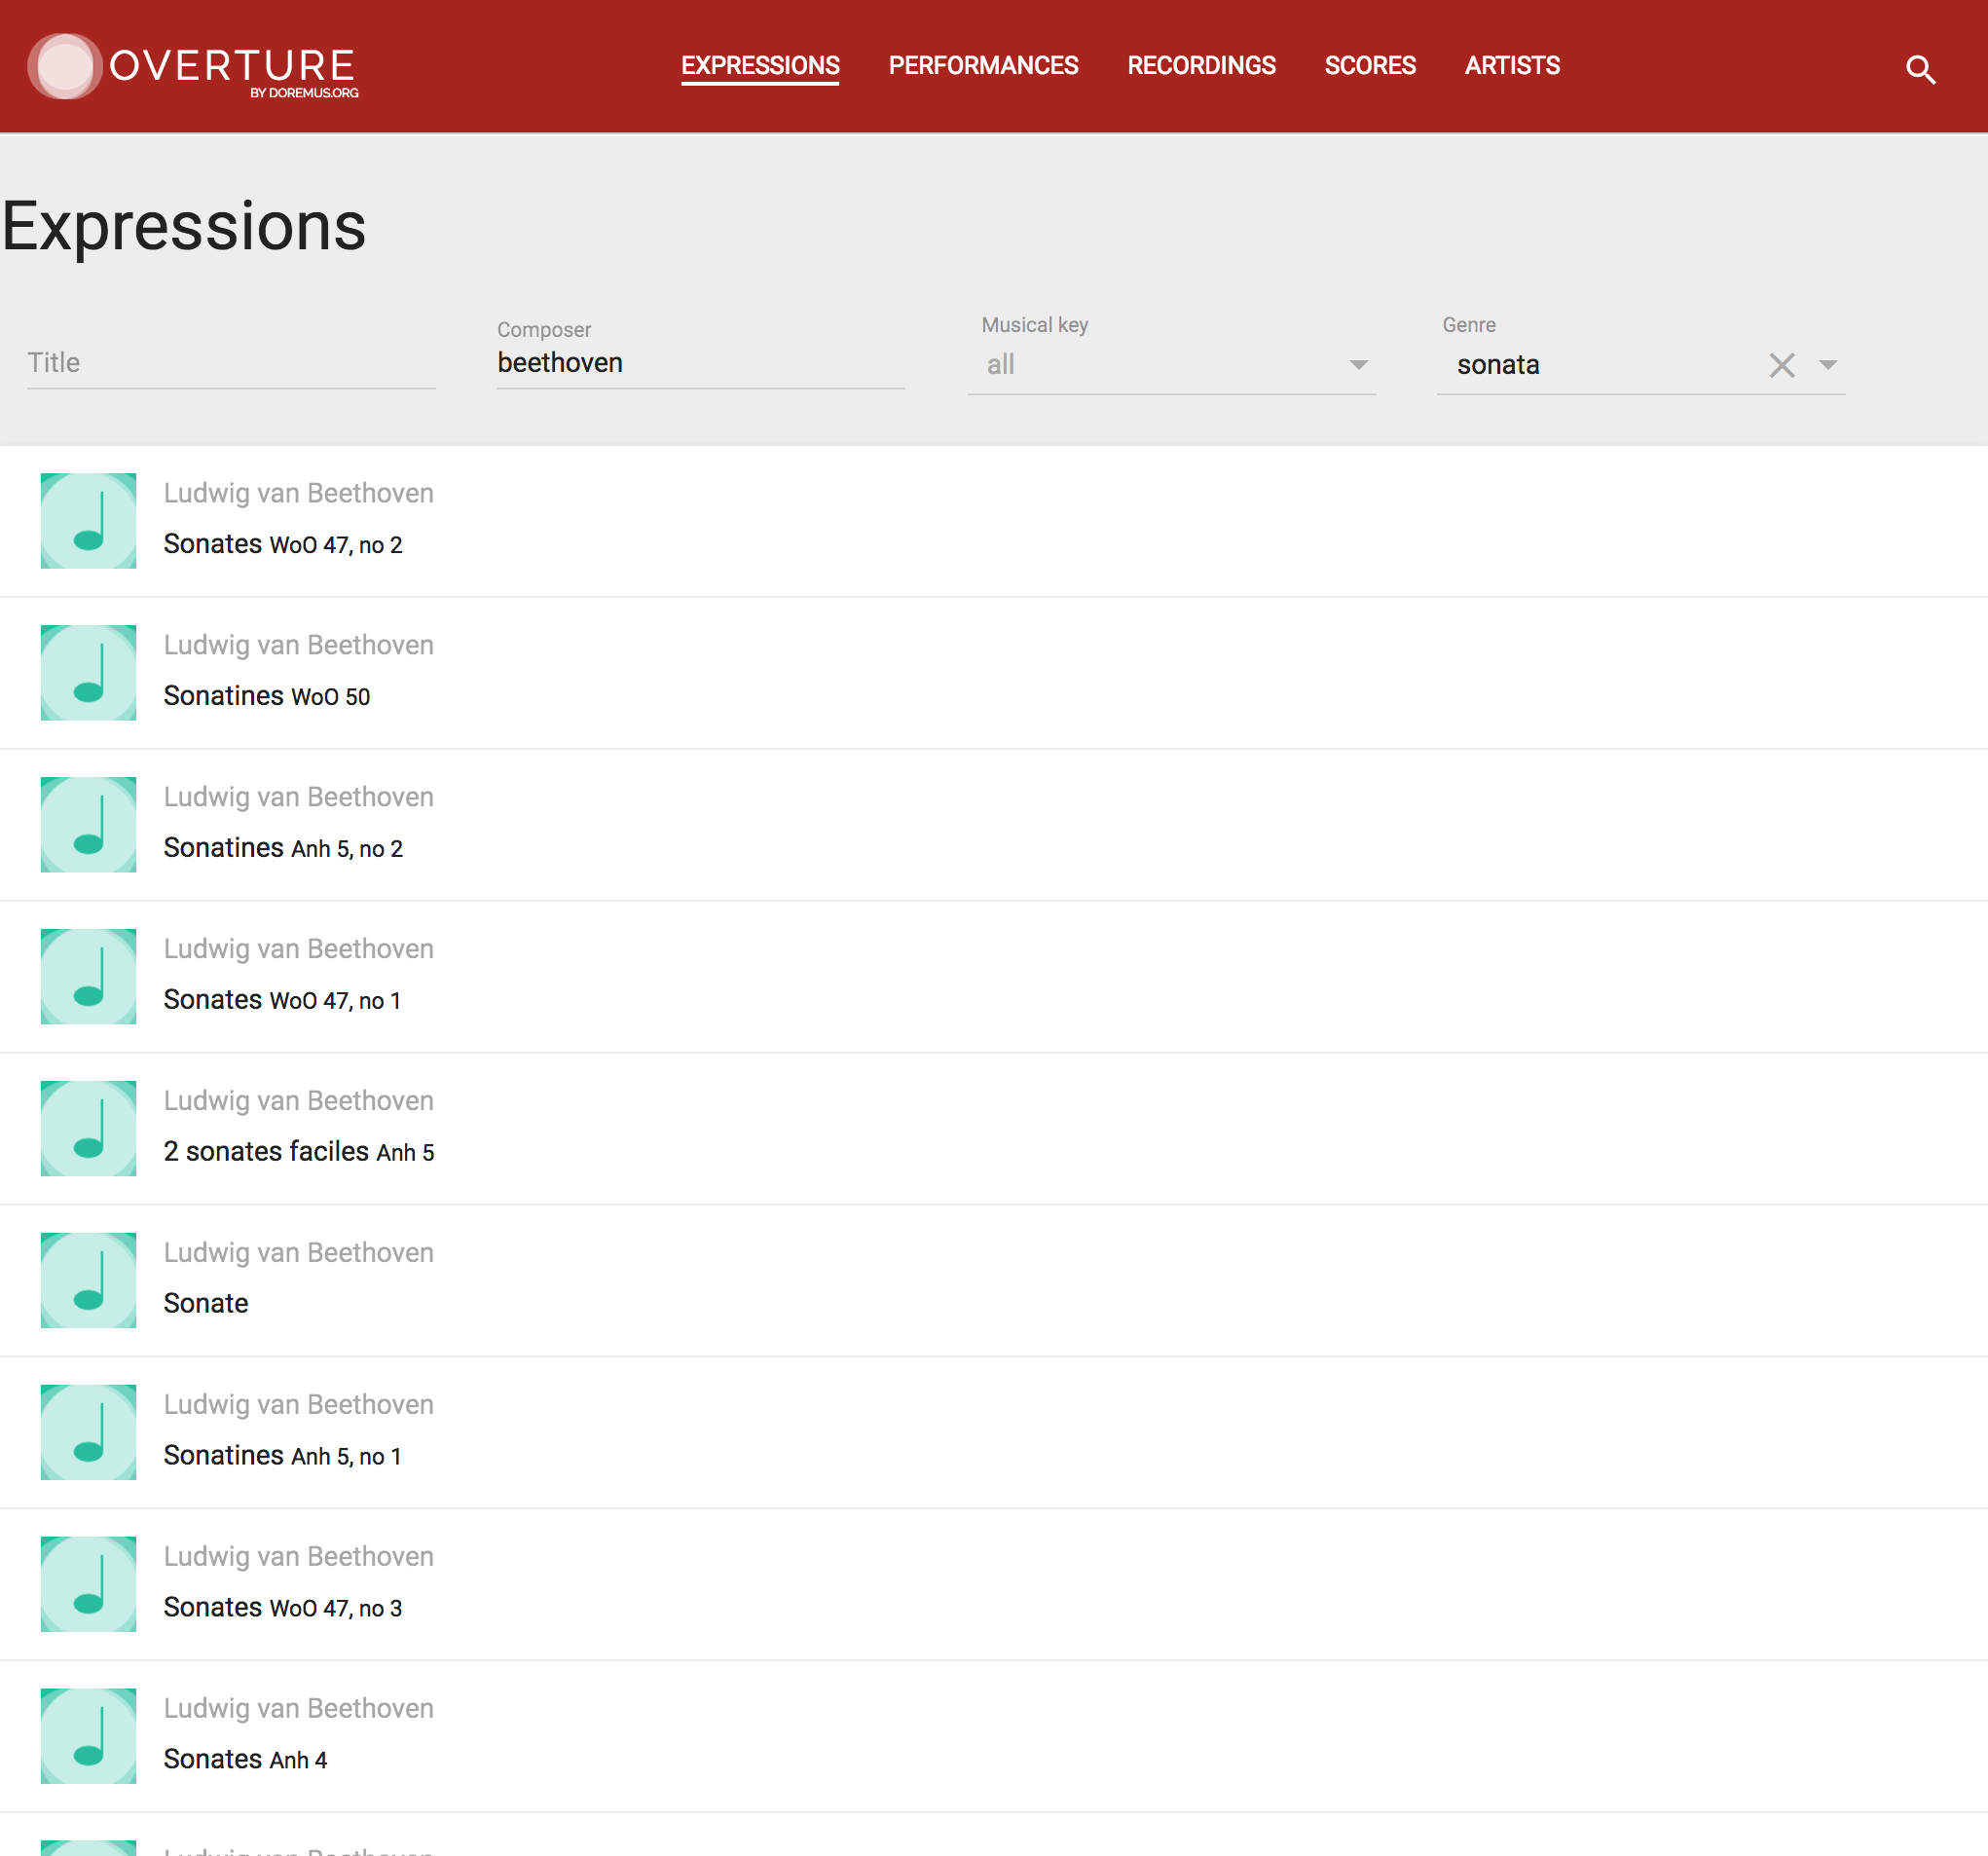
\includegraphics[width=\columnwidth]{figs/Overture_list.png}}}
%  \caption{The list of expressions in \textsc{Overture} filtered by composer and genre.}
%  \label{fig:overture-list}
% \end{figure}

The richness of the DOREMUS model offers to the end user the chance to perform a detailed advanced search and retrieve the list of the works that exactly match the chosen filters. All expressions are searchable by a large number of facets, that include the title and the composer, but also the key, the genre, the detailed casting. The use of hierarchical properties in the controlled vocabulary for genres and medium of performance, allows the smart retrieval not only of the entity that match exactly the chosen value (i.e. ``string''), but also any of its narrower concepts (i.e. ``violin'', ``cello'', etc.). The list of expression is automatically updated as soon as the user modifies the filter parameters.

An alternative way to discover the information in Overture is to follow links in every page of the application. Passing from an expression to its movements, from an artist to its works and from a performance to its recordings, will let the user to explore the data following the links in the same way they are in the graph. Also, certain properties can work as a bridge between entities, appearing clickable in the user interface.

A crucial task in multimedia application consists in the set up of a recommendation system, that automatically brings the user to new interesting elements, similar to the one currently displayed. We inserted a very simple recommendation section in the expression page, that suggests other expressions that have some properties in common with the current one, like the genre, the composer and the instruments foreseen. This part will host in future more sophisticated recommendation, that are possible using the richness of the data and the structure of RDF. 

%%%%%%%%%%%%%%%%%%%%%%%
%%%  6. Evaluation  %%%
%%%%%%%%%%%%%%%%%%%%%%%

\section{Evaluation}
\subsection{Model Evaluation}
The success of a model can be evaluated in its ability in providing answers to end-user questions. Before the beginning of the project, a list of questions have been collected from experts of the partner institutions\footnote{\url{https://github.com/DOREMUS-ANR/knowledge-base/tree/master/query-examples}}. These question can be related to practical use case (the search of all the scores that suit a particular formation), to musicologist topic (the music of a certain region in a particular historical period), to interesting stats (the works usually performed or published together), or to curious connection between works, performances or artists. Most of the questions are very specific and complex, so that it is very hard to find their answer using traditional search engines results.

We have grouped these questions in categories, according to the DOREMUS classes involved in the question. After this, we translated them in SPARQL queries that we run on the DOREMUS endpoint. We can distinguish 4 different cases:
\begin{enumerate}
 \item Questions that fit perfectly the model and the data and that can be readily converted as SPARQL queries (e.g. \textit{Retrieve all performances in which a composer interprets his or her works});
 \item Questions that fit the model but not yet the current state of the data since data conversion is still a work in progress. It is sometimes difficult to parse the source files when they contain plain text and not a regular syntax that enables to extract structured information (e.g. \textit{Retrieve the list of the works of which at least one of the dedicatees is also a performer of the work} can be retrieved only after a successful parsing of the plain text note about the dedication);
 \item Questions that overflow the model, because they contain aspects that go beyond the goal of the project (e.g \textit{Retrieve a list of works of chamber music composed in the 19\textsuperscript{th} century by Scandinavian composers} requires to know the birth place of the composer, and if this place is located in one of the Scandinavian countries). In fact, this kind of query can be solved by performing federated queries involving the Linked Open Data cloud (LOD) and in particular datasets such as Geonames or DBpedia, exploiting one of the advantages of Semantic Web technologies;
 \item Questions with an intrinsic complexity (e.g. \textit{Retrieve the works written for -- strictly / at least / at most -- violin, clarinet and piano}). Most of them are caused by the nature of the Semantic Web, that includes an Open World Assumption, and makes hard the formulation of queries that involves the check for the absence of a certain property. Despite this, we can anyway provide an answer to this query by considering only information contained in our database (Closed World Assumption).
\end{enumerate}

\tabref{tab:queries} provides an overview of how many queries we currently can write for each category. The implementation of recordings, scores, performance that is still work in progress -- along with the interconnection to the LOD repositories -- is one important reason for which some questions have not yet been translated into SPARQL and other ones have not results. 

\begin{table}
 \begin{center}
 \begin{tabular}{|l|c|}
  \hline
  Category & Query/ \\
    & Questions \\
  \hline
  A. Works & 23 / 29 \\
  \hline
  B. Artists & 1 / 3 \\
  \hline
  C. Performances & 6 / 9 \\
  \hline
  D. Recordings & 0 / 11 \\
  \hline
  E. Publications & 0 / 5 \\
  \hline
 \end{tabular}
\end{center}
 \caption{For each category of questions, we provide the ratio of the number of converted queries}
 \label{tab:queries}
\end{table}

% TODO integrate this queries in Overture.

\subsection{Linking with LEGATO} \label{sec:eval-link}
\begin{table*}[t]
\begin{center}
	\begin{tabular}{|c|c|c|c|c|c|c|c|c|c|}
		\hline
		{}{}{} & \multicolumn{3}{c|}{9-HT} & %
		\multicolumn{3}{c|}{4-HT} &  \multicolumn{3}{c|}{FP-trap}\\
		\cline{2-10}
		& F & P & R & F & P & R & F & P & R \\
		\hline
		\textbf{\textbf{LEGATO}} & 0.92 & 0.93 & 0.9 & 0.88 & 0.89 & 0.87 & 0.85 & 0.87 & 0.82 \\
		\hline
		\textbf{SILK} & 0.6 & 0.76 & 0.5 & - & - & - & 0.31 & 0.34 & 0.29\\
		\hline
	\end{tabular}
	\caption{Results on the DOREMUS benchmark data from the OAEI's instance matching track 2016}
	\label{table:doremus}
\end{center}
\end{table*}

We have evaluated the performance of our linking tool LEGATO, described in Section~\ref{subsec:datalinking}, by comparing it to a state-of-the-art tool, SILK, on the DOREMUS benchmark data that was published on the Instance Matching track of the annual OAEI campaign. Note that although the DOREMUS data has evolved since the publication of this benchmark in 2016, this evaluation is done on the publicly available OAEI datasets. This track consists of three datasets, described below. 

Nine heterogeneities (9-HT): This dataset consists of two small graphs from the BnF and the PP, containing about 40 instances each. The linking task consist in discovering 1:1 equivalence relations between them. There are 9 types of heterogeneities that these data manifest, that have been identified by the music library experts, such as multilingualism, differences in catalogs, differences in spelling, different degrees of richness of description, {\it etc.}

Four heterogeneities (4-HT): This track consists of two bigger datasets containing about 200 instances each, related by 1:1 equivalence relations. There are 4 types of heterogeneities that these datasets manifest: 1) Orthographical differences, 2) Multilingual titles, 3) Missing properties, 4) Missing titles.

The False Positives Trap (FP-trap): This task consists in correctly disambiguating the instances contained in two datasets, by discovering 1:1 equivalence relations between the instances that they contain. We have selected several groups of works with highly similar descriptions where there exist only one correct match in each group. The goal is to challenge the linking tools capacity to avoid the generation of false positives and match correctly works in the presence of highly similar but still distinct candidates.

SILK needs to be configured by pointing out the properties to use for the linking. Therefore, we have first ran a key selection and ranking algorithm, allowing to select automatically the properties that provide the best likelihood of discovering links between two datasets, as described in \cite{achichi2016automatic}. We have then used these properties to configure SILK, thus providing the ``best conditions'' for the tool to perform. The results of the comparison in terms of F-measure, Precision and Recall are given in Table \ref{table:doremus}. As we can see from the table, LEGATO outperforms SILK on all three tasks (no results are returned by SILK on the second task). 

\section{Conclusion and Future Work}
\label{sec:conclusion}
We proposed a complete workflow for the management of music metadata using Semantic Web technologies. The starting point is the realisation of a specialized ontology and a set of controlled vocabularies. Then, we proposed an approach for converting and interlinking data. Finally, we show how this data can be used in real web application, allowing the end user to explore the data and get music recommendation. Once the validation of vocabulary alignment will end, we will realise a pivot vocabularies for each categories, that contains all the concepts and the different labels that come from the different sources, in order to connect the whole knowledge graph.

On the data side, we are working on the improvement of the parsing of the data using Named Entity Recognition (NER) techniques, that will link also the DOREMUS data to external LOD datasets. Regarding the data linking task, although our results on the benchmark data are promising, we still need to address several scaling issues that will allow us to efficiently interconnect our datasets, containing sometimes hundreds of thousands of records. We will be also working on creating links form our data to well-established web knowledge graphs, such as DBpedia.

Finally, we are planning to integrate a series of interesting features in \textsc{Overture}, which include the integration of media like images and sound tracks, the retrieving of related information from LOD, and the realisation of a dashboard with interesting and unusual results (along the lines of the Wikipedia homepage). Moreover, a content-based recommendation system will be realised in order to exploit the richness of DOREMUS data. The recommendation results will be available through API and hosted in the web application.

%\section{Acknowledgments}
%TODO uncomment after review
%This work has been partially supported by the French National Research Agency (ANR) within the DOREMUS Project, under grant number ANR-14-CE24-0020.

% For bibtex users:
\bibliography{bib-doremus}

\end{document}
